\section{Raspberry Pi}
Der Raspberry Pi stellt in diesem Projekt unter anderem die Schnittstelle zum Web oder Internet dar. Für den Raspberry Pi sprachen einige Argumente.
\begin{itemize}
\item Es kann das gleiche Funkmodul wie für die Arduinos verwendet werden
\item Es ist eine große Community vorhanden
\end{itemize}
Ferner handelt es sich beim Raspberry Pi um einen Ein-Platinen-Rechner. 

\subsection{Hardware}
Bei dem Hauptprozessor des Raspberry Pi handelt es sich um einen Broadcom BCM2835. Die Architektur des Prozessors nennt sich \textit{ARM}. ARM hat einige Vorteile gegenüber x86 Prozessoren: 
\begin{itemize}
\item kleiner Energiebedarf
\item geringe Wärmeentwicklung
\subitem normalerweise keine Kühlung notwendig
\item kleine Bauweise
\end{itemize}

\subsubsection{Allgemein}
Die ARM-Architektur besitzt folgende Eigenschaften: 
\begin{itemize}
\item \ac{RISC}
\item 32-Bit Daten- und Adressbus
\item 7 Prozessor Modi
\item 37 Register
\item 5 Hauptadressierungsmodi
\item Datentypen
\subitem 32 Bit Wort
\subitem 16 Bit Halbwort
\subitem Byte (8 Bit)
\item Instruktionen
\subitem 54 ARM-Instruktionen, sie sind jeweils ein Wort
\subitem 38 Thumb-Instruktionen
\subitem Datenverarbeitungen werden auf Wörter angewandt
\end{itemize}

\subsubsection{Modi}
\begin{table}
    \begin{tabular}{lll}
    Modus          & Beschreibung                    & Ausnahme-Modus? \\ \hline
    User           & Ausführung normaler Programme   & nein            \\
    System         & privelegierter Modus            & nein            \\
    Supervisor     & Modus für Systemcalls           & ja              \\
    Abort          & Memory Abort                    & ja              \\
    Undefined      & Undefinierte Anweisung (Fehler) & ja              \\
    Interrupt      & Modus für Interrupts            & ja              \\
    Fast Interrupt & Modus für schnellen Interrupt   & ja              \\
    \end{tabular}
    \caption {ARM-Modi}
\end{table}
Ein Interrupt und ein Fast Interrupt unterscheiden sich in ihrer Priorität. Ein Fast Interrupt kann also einen Interrupt unterbrechen. Es darf jedoch nur ein Fast Interrupt zu einem Zeitpunkt auftreten. Der User-Modus ist der einzige Modus ohne Privilegien, die anderen Modi haben mehr Rechte wie der User-Modus. In User-Modus werden standardmäßig Programme ausgeführt. Einige Register sind Modussensitiv, soll heißen, dass sie nur in einem bestimmten Modus nutzbar sind. Wenn der Rechner startet, befindet sich der Prozessor im Supervisor-Modus. Später kann von jedem Modus aus gewechselt werden, außer aus dem User-Modus. Man kann ihn nur über einen Softwareinterrupt verlassen. 
\subsubsection{Register}
Im User-Modus kann man über die Register R0 bis R12 frei verfügen. Register R13 ist der Stackpointer, Register R14 das Linkregister. Das Linkregister merkt sich die Return-Adresse um nach einem Funktionsaufruf zurückzukehren. Das Register R15 ist wird als Programm-Counter genutzt.

\begin{figure}
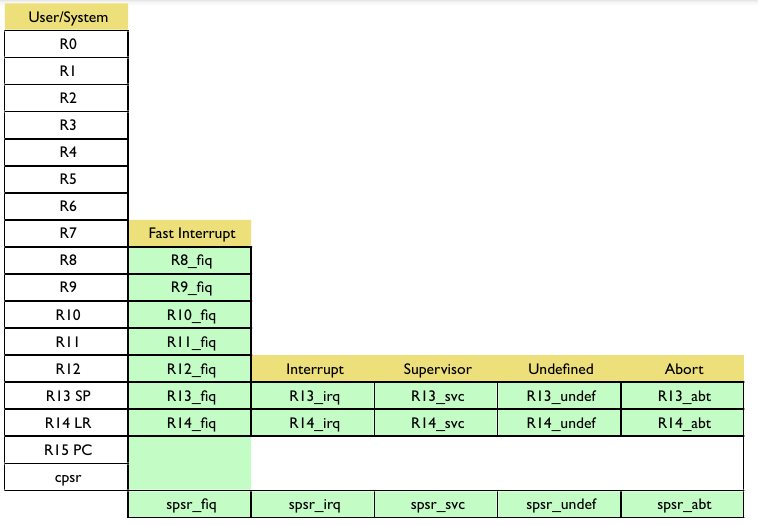
\includegraphics[width=\columnwidth]{bilder/overviewRegister} 
\caption{Überblick über die Register Quelle: arm-2009.pdf}
\label{Register}
\end{figure}

Das Statusregister ist im Detail wie folgt aufgebaut:
\begin{figure}
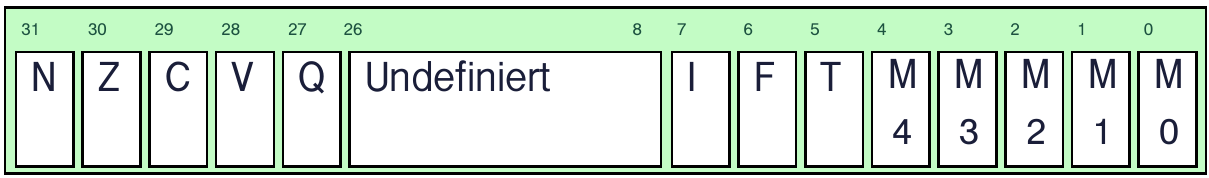
\includegraphics[width=\columnwidth]{bilder/statusRegister} 
\caption{Das Statusregister im Detail Quelle: arm-2009.pdf}
\label{Statusregister}
\end{figure}
 
Das hochwertigste Bit fungiert als Vorzeichen. Das 30. Bit ist bei Null gesetzt, das 29. Bit \textit{C} ist gesetzt, wenn das Ergebnis einer Operation eine Übertrag hat. Bit \textit{V} ist bei einem Overflow (Überlauf) gesetzt. Bit \textit{Q} fungiert bei ARM-Prozessoren, die als \ac{DSP} eingesetzt werden, als Überlaufbit für erweiterte Instruktionen. Die Bits 26 bis 8 sind undefiniert, Bit \textit{I} (7) ist das Interruptbit. Es ist bei einem Interrupt gesetzt. Bit \textit{F} (6) ist das Fast Interrupt-Bit. Es ist dementsprechend gesetzt. Das Bit \textit{T} (5) gibt den zeigt an, ob der Thumb-Mode aktiv ist. Im Thumb-Mode sind die Instruktionen nicht 32 Bit lang, sondern nur 16 Bit. Instruktionen im Thumb-Mode sind bieten demnach weniger Optionen. Sie arbeiten häufig implizit. Der Vorteil von Thumb-Instruktionen ist, dass die Instruktionen weniger Speicher benötigen. Die Abarbeitngsgeschwindigkeit von 32 Bit Instruktionen und Thumb-Instruktionen ist identisch. Die Bits 4 bis 0 kodieren den Modus der CPU:
\begin{table}
    \begin{tabular}{l|l}
    Bit M\textsubscript{4}, ..., M\textsubscript{0}  & Modus          \\ \hline
    10000 & User           \\
    10001 & Fast Interrupt \\
    10010 & Interrupt      \\
    10011 & Supervisor     \\
    10111 & Abort          \\
    11011 & Undefined      \\
    11111 & System         \\
    \end{tabular}
    \caption {Modi im ARM Statusregister}
\end{table}
TODO Quelle: arm-2009.pdf

\subsubsection{Memory Management Unit}
ARM-Prozessoren verfügen wie auch x86-Prozessoren über eine \ac{MMU}. Dieser Hardware-Baustein hat die Aufgabe virtuelle Speicheradressen in reale Speicheradressen zu übersetzten. Dies hat mehrere Vorteile: 
\begin{itemize}
\item einfacherer Umgang mit Adressen
\item Erhöhung der Sicherheit 
\item keine großen, ungenutzten Speicherstellen am Stück 
\end{itemize}

\begin{figure}
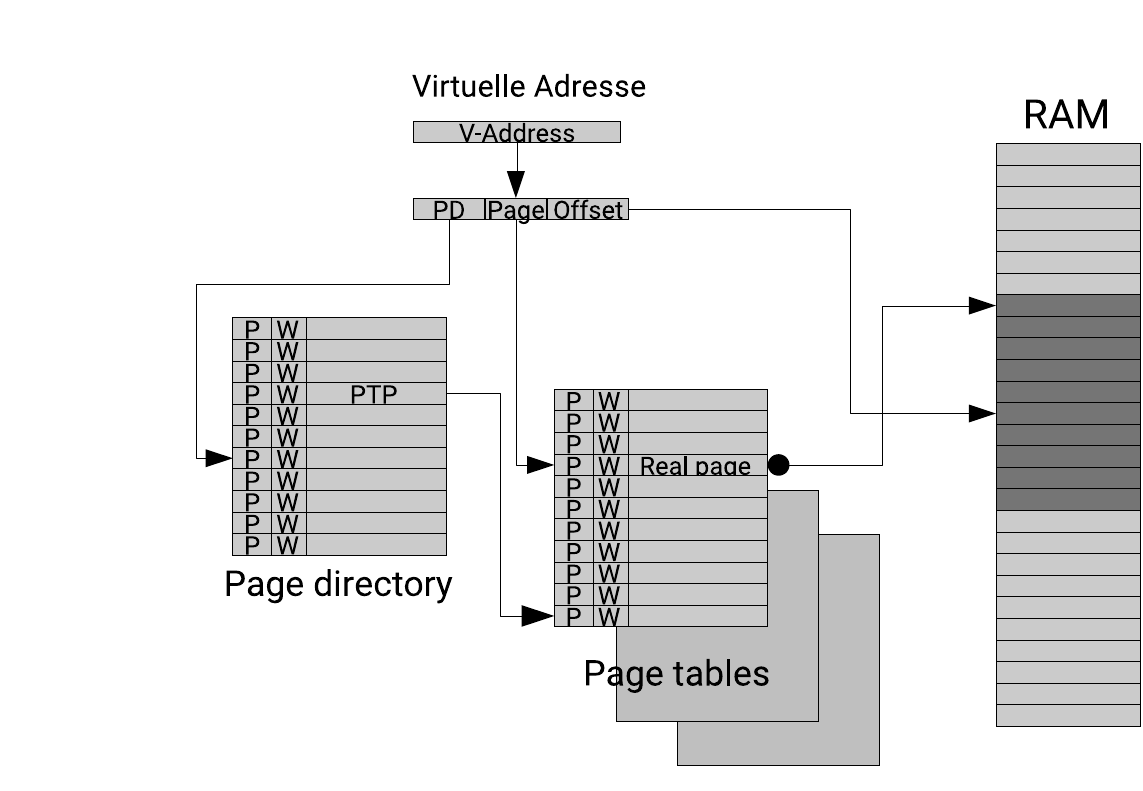
\includegraphics[scale=0.3]{bilder/mmu} 
\caption{Virtuelle Adressierung Quelle: Richter}
\label{MMU}
\end{figure}

Die Virtuelle Adresse (V-Address) besteht (vereinfacht) aus einer Adresse für das Page Directory, der Adresse für die eigentliche Page und dem Offset innerhalb der Page. \textit{P} und \textit{W} in der Abbildung sind Bits. Ist das \textit{P}-Bit gesetzt, so ist die jeweilige Seite im Hauptspeicher verfügbar. Ist das \textit{W}-Bit gesetzt, so darf auf die Page geschrieben werden. Das \textit{W}-Bit ist für weitere Mechanismen notwendig. Diese sind jedoch nicht Gegenstand dieser Arbeit.  

Dadurch, dass der Prozessor nicht mit realen Adressen arbeiten muss, muss der Programmierer oder Compiler die konkreten realen Adressen nicht kennen. Nun ist es möglich zu realisieren, dass es für Programme so aussieht, als wäre der zugeteilte Speicherbereich am Stück. Physikalisch ist der zugewiesene Speicher jedoch über den ganzen RAM verteilt. Ferner ist es auch der Fall, dass ein Betriebssystem ständig Programme startet und beendet. Endet ein Programm, so muss man den allokierten   Speicherbereich wieder dellokieren. Die virtuelle Adressierung verhindert in diesem Zusammenhang, dass groß Speicherbereiche "brach" liegen. Würde man kein virtuelle Adressierung verwenden, so ist nach dem Ende eines Programmes, dass 1 Gb Speicher benutzt hat, eine 1 Gb große Lücke im Speicher. Dieser Umstand kann zu Problemen führen, wenn ein neues Programm startet und viel Speicher benötigt. Im Falle der virtuellen Adressierung ist es irrelevant, ob der angeforderte Speicher am Stück ist oder ob die benutzen Speicherstellen über den RAM verteilt sind.    

TODO Quelle: Richter

\subsubsection{Externe Anschlüsse}
Der Raspberry Pi verfügt über mehrere physikalische Schnittstellen. 
\begin{itemize}
\item \ac{GPIO}
\item USB
\item 3,5 mm Klinke für Audio
\item \ac{CSI}
\item RJ45 für Ethernet
\item HDMI
\item \ac{DSI}
\end{itemize}

Die \ac{GPIO}-Pins ermöglichen unter anderem eine Kommunikation über \ac{I2C} und den \ac{SPI}. 

TODO Quelle: Rasi Handbuch
 
\subsection{Software}
Dieses Unterkapitel betrachtet 
 
TODO Exceptions und Assembler hier (aus arm-2009)





          
 
